% This text is a supplement of CINTA.
% May. 2018
% Author: Libin Wang
% SCNU
% additional use of \usepackage{beamerthemesplit}
\documentclass{beamer}

%%%%%%%%%%%%%%%%%%%%%%%%%%%%%%%%%%%%%%%%%%%%%%%%%%%%%%%%%%%%%%%%%%%%%
\usepackage{xeCJK}
%\usepackage[CJKbookmarks]{hyperref}

%% Support Chinese with TeX Live fonts.

\setCJKmainfont[
  BoldFont=FandolHei-Regular.otf,
  ItalicFont=FandolKai-Regular.otf,
  BoldItalicFont=FandolKai-Regular.otf
]{FandolSong-Regular.otf}
\setCJKsansfont[AutoFakeBold, AutoFakeSlant]{FandolHei-Regular.otf}
\setCJKmonofont{FandolFang-Regular.otf}

\setmainfont{Times New Roman} % 设置默认英文衬线字体

\setCJKfamilyfont{ls}{FandolSong-Regular.otf} %定义字体
%%%%%%%%%%%%%%%%%%%%%%%%%%%%%%%%%%%%%%%%%%%%%%%%%%%%%%%%%%%%%%%%%%%%%
\usepackage{tikz}
\usetikzlibrary{arrows.meta}

%\usepackage{beamerthemesplit} % new 
\usepackage{beamerthemeshadow}
\setbeamertemplate{headline}{}
\setbeamertemplate{footline}{}
\setbeamertemplate{navigation symbols}{}
\usepackage{amsmath, amsfonts, amssymb}

%% Setup for Code
\usepackage{listings}
\lstset{language = Python,
	showstringspaces = false,
	columns = fullflexible,
	numbers = left,
	numberstyle = \tiny,
	frame = single}

\newtheorem{proposition}[theorem]{Proposition}
\newtheorem{remark}[theorem]{Remark}
\newtheorem{claim}[theorem]{Claim}

\newcommand{\Grp}[1]{\mathbb{#1}}
%\title{A Concrete Introduction to Number Theory and Algebra-- 群同构、群同态与商群} 
\title{Mathematics for Computer Science -- Isomorphism, Homomorphism and Quotient Group.} 
\author{Libin Wang} 
\institute{School of Computer Science, South China Normal University}
\date{\today} 

\begin{document}

\frame{\titlepage} 

\frame{\frametitle{Table of contents}\tableofcontents} 

\section{Isomorphisms} 
\frame{\frametitle{本章概览.} 

\begin{exampleblock}{学习思路.}
本章有一条联系紧密的知识链：从同态、同构出发，经过Kernel、正规子群、商群等，最后到达同构定理。而这整条知识链围绕着一个核心目标：考察群结构。
\end{exampleblock}

}

\frame{\frametitle{Isomorphisms(同构.)} 

\begin{block}{Motivation.}
Many groups may have different appearances, however they are essentially same.
\end{block}

}

\frame{\frametitle{Isomorphisms(同构).} 
\begin{block}{Definition of Isomorphism.}
	Two group $(\mathbb{G}, \cdot)$ and $(\mathbb{H}, \circ)$ are isomorphic if there exists a one-to-one and onto map $\phi: \mathbb{G} \mapsto \mathbb{H}$ such that the group operation is preserved; that is,
	$$\phi(a \cdot b) = \phi(a)\circ \phi(b)$$
	for all $a$ and $b$ in $\mathbb{G}$. If $\mathbb{G}$ is isomorphic to $\mathbb{H}$, we write $\mathbb{G}\cong \mathbb{H}$. The map $\phi$ is called an isomorphism.
\end{block}
	
}

\frame{\frametitle{Examples of Isomorphisms.} 
\begin{example}
$\mathbb{Z}_4\cong \langle i \rangle$, since we can define a bijective map $\phi: \mathbb{Z}_4 \mapsto \langle i \rangle$ by $\phi(n) = i^n$. The map $\phi$ is one-to-one and onto, since
\begin{align*}
\phi(0) &= 1\\
 \phi(1) &= i\\
 \phi(2) &= -1\\
 \phi(3) &= -i.
\end{align*}
Moreover, $\phi$ preserves the group operation, since
\[ \phi(m+n) = i^{m+n} = i^m i^n = \phi(m) \phi(n).\]
\end{example}
}

\frame{\frametitle{Examples of Isomorphisms.} 
	\begin{exampleblock}{Isomorphic groups.}
		Since $\mathbb{Z}_8^* = \{1, 3, 5, 7 \}$, $\mathbb{Z}_{12}^* = \{1, 5, 7, 11 \}$, we can 
		find an isomorphism $\phi$ to show that:
		$$\mathbb{Z}_8^* \cong \mathbb{Z}_{12}^* $$
			An isomorphism $\phi : \mathbb{Z}_8^*  \mapsto \mathbb{Z}_{12}^*$ is defined by :
				\begin{align*}
				1 &\mapsto 1 \\
				3 &\mapsto 5 \\
				5 &\mapsto 7\\
				7 &\mapsto 11
				\end{align*}
		Can you find another isomorphism between these two groups?
	\end{exampleblock}
	
	\begin{alertblock}{(Question.)}
		Is $\mathbb{Z}_{61}^*$ isomorphic to $\mathbb{Z}_{77}^*$? Why or why not?
	\end{alertblock}
}

\frame{\frametitle{Examples of Isomorphisms.} 
	
	
	\begin{block}{Question-1.}
		Is $\mathbb{Z}_{n}$ isomorphic to $\mathbb{U}_{n}$? Why or why not?
	\end{block}
	\pause
    \begin{block}{Question-2.}
		Is $\mathbb{Z}_{61}^*$ isomorphic to $\mathbb{Z}_{77}^*$? Why or why not?
	\end{block}
}

\frame{\frametitle{Theorem about Isomorphisms.} 
\begin{proposition}
\label{prop:iso_pr}
Let $\phi: \mathbb{G} \mapsto \mathbb{H}$ be an isomorphism of two groups, then the following statements are true.
\begin{enumerate}
\item $\phi^{-1}: \mathbb{H} \mapsto \mathbb{G}$ is an isomorphism;

\item $\vert \mathbb{G} \vert = \vert \mathbb{H} \vert $; 

\item If $\mathbb{G}$ is abelian, then $\mathbb{H}$ is abelian;

\item If $\mathbb{G}$ is cyclic, then $\mathbb{H}$ is cyclic;

\item if $\mathbb{G}$ has a subgroup of order $n$, then $\mathbb{H}$ has a subgroup of order $n$.
\end{enumerate}
\end{proposition}
\begin{proof}
Left as an exercise.
\end{proof}
}

\frame{\frametitle{Theorem about Isomorphisms.} 
     \begin{theorem}
     All cyclic groups of infinite order are isomorphic to $\mathbb{Z}$.	
     \end{theorem}
 \begin{proof}
 	Suppose $\mathbb{G}$ is a cyclic group with infinite order, and $g\in \mathbb{G}$ is a generator. Define $\phi: \mathbb{Z} \mapsto \mathbb{G}$ by $\phi: n \mapsto g^n$. Then
 	$$\phi(m+n) = g^{m+n} = g^m g^n = \phi(m)\phi(n).$$
 	Show $\phi$ is a bijective map. Left as an exercise.
 \end{proof}
}

\frame{\frametitle{Theorem about Isomorphisms.} 
	\begin{theorem}
		If $\mathbb{G}$ is a cyclic group of order $n$, then $\mathbb{G}$ is isomorphic to $\mathbb{Z}_n$.	
	\end{theorem}
	\begin{proof}
		Let $\mathbb{G}$ be a cyclic group with order $n$, generated by $g$. Define $\phi: \mathbb{Z}_n \mapsto \mathbb{G}$ by $\phi: k \mapsto g^k$, where $0 \leq k < n$. 
		Show $\phi$ is an isomorphism. Left as an exercise.
	\end{proof}
}

\frame{\frametitle{Theorem about Isomorphisms.} 
	\begin{corollary}
		If $\mathbb{G}$ is a cyclic group of order $p$ where $p$ is a prime, then $\mathbb{G}$ is isomorphic to $\mathbb{Z}_p$.	
	\end{corollary}
	\begin{proof}
		Easy!
	\end{proof}
}

\frame{\frametitle{Example.} 
	
	\begin{exampleblock}{单位根群.}
		$\mathbb{U}_n$与$\mathbb{Z}_n$同构！请问，令$n = p - 1$，$\mathbb{U}_n$与$\mathbb{Z}^*_p$同构吗？这个答案揭示了什么信息？
	\end{exampleblock}
}

\frame{\frametitle{Theorem about Isomorphisms.} 
	\begin{theorem}
		The isomorphism of groups determines an equivalence relation on the class of all groups.
	\end{theorem}
	\begin{proof}
	 Left as an exercise.
	\end{proof}
}

\frame{\frametitle{Theorem about Isomorphisms.} 
	\begin{theorem}{(Cayley)}
		Every group is isomorphic to a group of permutations.
	\end{theorem}
	\begin{proof}
		Omitted. Note that, it is important.
	\end{proof}
}

\frame{\frametitle{关于Isomorphisms的提醒.} 
	
	\begin{alertblock}{提醒.}
		同构是研究群结构的目标！
	\end{alertblock}
	\pause

	\begin{alertblock}{提问.}
		同态的目标是什么？
	\end{alertblock}
}

\section{Homomorphisms} 

\frame{\frametitle{Homomorphisms.（同态）}
\begin{block}{Definition of Homomorphism.}
	Two group $(\mathbb{G}, \cdot)$ and $(\mathbb{H}, \circ)$ are homomorphic if there exists a map $\phi: \mathbb{G} \mapsto \mathbb{H}$ such that the group operation is preserved; that is,
	$$\phi(a \cdot b) = \phi(a)\circ \phi(b)$$
	for all $a$ and $b$ in $\mathbb{G}$. The map $\phi$ is called a homomorphism.
\end{block}

\begin{alertblock}{(Basic idea.)}
	We relax the requirement that an isomorphism of groups be bijective, we have a homomorphism.
\end{alertblock}
}

\frame{\frametitle{Examples of Homomorphisms.}
        \begin{example}
              $\mathbb{Z}$是加法群，定义映射$\phi : \mathbb{Z} \mapsto \mathbb{Z}$为$\phi(k) = 2k$，$\forall k \in \mathbb{Z}$。
              可以验证$\phi$是一种群同态，因为
              $$ \phi(i + j ) = 2(i +j) = 2i + 2j = \phi(i)+ \phi(j)$$
              $\phi$把整数映射为偶数。偶数在加法下成群。
        \end{example}
}

\frame{\frametitle{Examples of Homomorphisms.}
	\begin{exampleblock}{Example of Homomorphisms.}
		Let $\mathbb{G}$ be a group and $g\in \mathbb{G}$. Define a map $\phi : \mathbb{Z} \mapsto \mathbb{G}$ by $\phi(n) = g^n$. Then $\phi$ is a group homomorphism, since
		$$\phi(m+n) = g^{m+n} = g^m g^n = \phi(m) \phi(n).$$
		This homomorphism maps $\mathbb{Z}$ onto the cyclic subgroup of $\mathbb{G}$ generated by $g$.
	\end{exampleblock}
}

\frame{\frametitle{Examples of Homomorphisms.}
\begin{example}
        设$p$为素数，定义映射$\phi : \mathbb{Z}_p^* \mapsto \mathbb{Z}_p^*$为$\phi(g) = g^2$，$\forall g\in\mathbb{Z}_p^*$。
        可验证，$\phi$是一种同态映射，因为对任意的$g_1, g_2 \in \mathbb{Z}_p^*$满足：
        $\phi(g_1 g_2) = (g_1 g_2 )^2 =  g_1^2 g_2^2 = \phi(g_1) \phi(g_2)$。
\end{example}
}

\iffalse
\frame{\frametitle{Examples of Homomorphisms.}
	\begin{exampleblock}{Exercise.(Hint: Programming is permitted.)}
				Let $p$ be a prime, and $g\in \mathbb{Z}_p^*$. Define a map $\phi : \mathbb{Z} \mapsto \mathbb{Z}_p^*$ by $\phi(n) = g^n$, then $\phi$ is a group homomorphism.
				\begin{itemize}
					\item Given a specific $g\in \mathbb{Z}_p^*$, please find a homomorphism $\phi$ maps $\mathbb{Z}$ onto the cyclic subgroup of $\mathbb{Z}_p^*$ generated by $g$, and explicitly constructe the cyclic subgroup $\mathbb{H}$.
					
					\item Can you find a homomorphism maps $\mathbb{Z}_p^*$ onto the cyclic subgroup $\mathbb{H}$ generated by $g$? 
				\end{itemize}
	\end{exampleblock}
}
\fi


\frame{\frametitle{Normal subgroups（正规子群）.}
	\begin{block}{Definition of normal subgroups.}
		A subgroup $\mathbb{H}$ of a group $\mathbb{G}$ is normal in $\mathbb{G}$ if $g\mathbb{H} = \mathbb{H}g$ for all $g \in \mathbb{G}$.
	\end{block}
	
	\begin{alertblock}{(Basic idea 1.)}
		A normal subgroup is a subgroup that the right cosets and the left cosets are precisely the same, and $g\mathbb{H} = \mathbb{H}g$ represents a kind of "commutativity(交换性)".
	\end{alertblock}\pause
	  
	\begin{alertblock}{(Basic idea 2.)}
	A subgroup $\mathbb{H}$ of a group $\mathbb{G}$ is normal in $\mathbb{G}$ iff $\forall g\in \mathbb{G}$, $g\mathbb{H} g^{-1} \subseteq \mathbb{H}$. Moreover, for all $\forall g\in \mathbb{G}$,  $g\mathbb{H} g^{-1} = \mathbb{H}$
    \end{alertblock}

}

\frame{\frametitle{Basic Properties of Normal Subgroup.}
\begin{proposition}
Let $\mathbb{G}$ be a group and $\mathbb{H}$ be a subgroup of $\mathbb{G}$. Then the following statements are equivalent.
\begin{enumerate}
\item The subgroup $\mathbb{H}$ is a normal subgroup of $\mathbb{G}$, namely, $g\mathbb{H} = \mathbb{H}g$ for all $g \in \mathbb{G}$.

\item For all $g \in \mathbb{G}$, $g\mathbb{H}g^{-1} = \mathbb{H}$.
\end{enumerate}
\end{proposition}

}

\frame{\frametitle{Basic Properties of Normal Subgroup.}

\begin{proof}{(Proof of last proposition--1.)}
$(1)  \Rightarrow (2).$  Since $\mathbb{H}$ is a normal subgroup of $\mathbb{G}$, $g\mathbb{H} = \mathbb{H}g$ for all $g \in \mathbb{G}$. 
Hence, for a given $g\in \mathbb{G}$ and $h \in \mathbb{H}$, there exists an $h' \in \mathbb{H}$ such that $gh=h'g$. Therefore, $ghg^{-1} = h' \in \mathbb{H}$ 
or $g\mathbb{H}g^{-1} \subseteq \mathbb{H}$.  For $h \in \mathbb{H}$, $g^{-1}hg = g^{-1}h(g^{-1})^{-1} \in \mathbb{H}$. 
Hence, $g^{-1}hg = h'$ for some $h' \in \mathbb{H}$. Therefore, $h = gh′g^{-1} \in g\mathbb{H}g^{-1}$, namely, $\mathbb{H} \subseteq g\mathbb{H}g^{-1}$.  

\end{proof}
}

\frame{\frametitle{Basic Properties of Normal Subgroup.}

\begin{proof}{(Proof of last proposition--2.)}

$(2) \Rightarrow (1).$ Suppose that for all $g \in \mathbb{G}$, $g\mathbb{H}g^{-1} = \mathbb{H}$. 
Then for any $h \in \mathbb{H}$ there exists an $h'\in \mathbb{H}$ such that $ghg^{-1} = h'$. Consequently, $gh = h'g$ which means $g\mathbb{H}\subseteq \mathbb{H}g$. 
Similarly, we can prove that $\mathbb{H}g \subseteq g\mathbb{H}$.
\end{proof}
}

\frame{\frametitle{Basic Properties of Homomorphisms.}
	\begin{proposition}{Proposition 1.}
		Let $\phi : \mathbb{G}_1 \mapsto \mathbb{G}_2$ be a homomorphism of groups. Then
		\begin{enumerate}
			\item If $e$ is the identity of $\mathbb{G}_1$, then $\phi(e)$ is the identity fo $\mathbb{G}_2$;
			
			\item For any element $g \in \mathbb{G}_1$, $\phi(g^{-1}) = \lbrack \phi(g)\rbrack^{-1}$;
			
			\item If $\mathbb{H}_1$ is a subgroup of $\mathbb{G}_1$, then $\phi(\mathbb{H}_1)$ is a subgroup of $\mathbb{G}_2$;
			
			\item If $\mathbb{H}_2$ is a subgroup of $\mathbb{G}_2$, then $\phi^{-1}(\mathbb{H}_2)$ is a subgroup of $\mathbb{G}_1$. Furtheremore, if $\mathbb{H}_2$ is normal in $\mathbb{G}_2$, then $\phi^{-1}(\mathbb{H}_2)$ is normal in $\mathbb{G}_1$.
		\end{enumerate}
	\end{proposition}
	
	\pause
	
	\begin{proof}
		Omitted. 
	\end{proof}
}

\frame{\frametitle{Basic Properties of Homomorphisms.}
	
	\begin{definition}{(Definition of Kernel.)}
	   	Let $\phi : \mathbb{G} \mapsto \mathbb{H}$ be a group homomorphism and $e$ is the identity of $\mathbb{H}$. By previous proposition, $\phi^{-1}(\{ e \})$ is subgroup of $\mathbb{G}$. This subgroup is called the kernel of $\phi$ and denoted by $\operatorname{Ker} \phi$.
	\end{definition}
	
	\pause
   	\begin{example}
   	        设$p$为素数，同态映射$\phi : \mathbb{Z}_p^* \mapsto \mathbb{Z}_p^*$定义为$\phi(g) = g^2$，$\forall g\in\mathbb{Z}_p^*$。
   	        可验证，$\phi $把$\{1, p-1\}$映射为
   	        群$\phi(\mathbb{Z}_p^*)$的单位元$1$，所以$\operatorname{Ker} \phi = \{1, p-1\}$。
   	\end{example}
}


\frame{\frametitle{Basic Properties of Homomorphisms.}
	
	\begin{proposition}{(Kernel.)}
		Let $\phi : \mathbb{G} \mapsto \mathbb{H}$ be a group homomorphism. Then the kernel of $\phi$ is a normal subgroup of $\mathbb{G}$.
	\end{proposition}
	
	\pause
	
	\begin{proof}
		 Trivial. Since the trivial subgroup of $\mathbb{H}$ is normal.
	\end{proof}
}

\frame{\frametitle{关于Homomorphisms的提醒.} 
	
	\begin{alertblock}{提醒}
		同态是研究群结构的重要手段：通过群同态去找正规子群，即同态映射的Kernel.
	\end{alertblock}
}
\frame{\frametitle{习题.}
\begin{block}{习题.}
\begin{itemize}
\item 如果$\mathbb{H}_1$和$\mathbb{H}_2$是群$\mathbb{G}$的正规子群，
证明$\mathbb{H}_1 \mathbb{H}_2$也是群$\mathbb{G}$的正规子群。

\item 证明，$\mathbb{H}$是$\mathbb{G}$的正规子群
当且仅当对任意$g \in \mathbb{G}$，$g\mathbb{H}g^{-1} \subseteq \mathbb{H}$。
%AATA

\item 定义映射$\phi: \mathbb{G}\mapsto \mathbb{G}$为：$g \mapsto g^2$。请证明$\phi$是一种群同态当且仅当$G$是阿贝尔群。

\item 设$\phi: \mathbb{G}\mapsto \mathbb{H}$是一种群同态。请证明：如果$\mathbb{G}$是循环群，
则$\phi(\mathbb{G})$也是循环群；如果$\mathbb{G}$是交换群，则$\phi(\mathbb{G})$也是交换群。
 \end{itemize}
 \end{block}
 }
\section{Quotient group}

\frame{\frametitle{Quotient Groups(商群).}
\begin{theorem}
If $\mathbb{H}$ is a normal subgroup of a group $\mathbb{G}$, then the cosets of $\mathbb{H}$ in $\mathbb{G}$ form a group $\mathbb{G}/ \mathbb{H}$ 
under the operation $(a \mathbb{H}) (b \mathbb{H}) = ab \mathbb{H}$. This group is call the \emph{quotient group} or \emph{factor group} of $\mathbb{G}$ and $\mathbb{H}$.
\end{theorem}\pause

\begin{alertblock}{Understand the operation.}
	How to understand the operation $(a \mathbb{H}) (b \mathbb{H}) = ab \mathbb{H}$?\pause
	
	Since $\mathbb{H}$ is normal, then:
	$$(a \mathbb{H}) (b \mathbb{H}) = (\mathbb{H}a) (b \mathbb{H}) = (a b \mathbb{H}) \mathbb{H} = ab \mathbb{H}$$
\end{alertblock}
}

\frame{\frametitle{进一步理解商群的群操作.}

\begin{block}{Understand the operation.}
	To understand the operation $(a \mathbb{H}) (b \mathbb{H}) = ab \mathbb{H}$, we show that since $\mathbb{H}$ is normal, then:
	$$(a \mathbb{H}) (b \mathbb{H}) = (\mathbb{H}a) (b \mathbb{H}) = (a b \mathbb{H}) \mathbb{H} = ab \mathbb{H}$$ \pause
	
	使用了两种属性：
	\begin{itemize}
	\item 正规子群的“交换性”
	
	\item 结合律
	\end{itemize}
\end{block}\pause

\begin{alertblock}{另一种理解.}
有没有另一种理解方式？借助正常的思维(什么是正常思维？)与底层定义（直接借助群元素的操作！）。
\end{alertblock}

}

\frame{\frametitle{进一步理解商群的群操作.}

\begin{block}{正常思维！}
	我们需要证明$(a \mathbb{H}) (b \mathbb{H}) = ab \mathbb{H}$，即我们需要证明：
	\begin{itemize}
		\item $(a \mathbb{H}) (b \mathbb{H}) \subseteq ab \mathbb{H}$
		
		\item $ab \mathbb{H} \subseteq (a \mathbb{H}) (b \mathbb{H}) $
		\end{itemize} 
\end{block}\pause

\begin{proof}
要证明 $(a \mathbb{H}) (b \mathbb{H}) \subseteq ab \mathbb{H}$，即任取$a h_1 b h_2 \in a \mathbb{H} b \mathbb{H}$，
证$a h_1 b h_2 \in ab \mathbb{H}$。但是，这是容易的，因为：
\begin{align*}
	a h_1 b h_2 &= h_3 a b h_2  \\
	&= ab h_4 h_2\\
	&= ab h_5  \in  ab \mathbb{H}
	\end{align*}
	
另一个方向，证明$ab \mathbb{H} \subseteq (a \mathbb{H}) (b \mathbb{H}) $则留给大家作为练习。	
\end{proof}
}

\frame{\frametitle{Theorem of Quotient Groups.}
\begin{theorem}{(Quotient Groups).}
If $\mathbb{H}$ is a normal subgroup of a group $\mathbb{G}$, then the cosets of $\mathbb{H}$ in $\mathbb{G}$ form a group $\mathbb{G}/ \mathbb{H}$ of order $\lbrack \mathbb{G}: \mathbb{H}\rbrack$.
\end{theorem}
}

\frame{\frametitle{Theorem  of Quotient Groups.}
	\begin{proof}{(Basic ideas.)}
		\begin{enumerate}
			\item What is the group operation? $(a \mathbb{H})(b \mathbb{H}) = ab \mathbb{H}$\pause
			
			\item Prove this operation is well-defined, i.e.,the group operation must be independent of the choice of coset representative. Let $a \mathbb{H} = b \mathbb{H}$, $c \mathbb{H} = d\mathbb{H}$. We must prove that
			\[(a\mathbb{H})(c\mathbb{H}) = a c\mathbb{H} = bd \mathbb{H} = (b\mathbb{H})(d\mathbb{H})\]\pause	
			
			\item Why we need "well-defined"? \pause
			
			\item Check the axioms of group. Easy!
		\end{enumerate}
	\end{proof}
}

\frame{\frametitle{Theorem  of Quotient Groups.}
\begin{remark}{(良定义操作.)}
所谓良定义的操作，
就是要求操作独立于所参与操作的\emph{代表元}。比如，对任意群$\mathbb{G}$和其上的某种操作$\psi: \mathbb{G}\mapsto \mathbb{G}$，
要求$\psi$良定义就是要求对任意的群元$a, b\in \mathbb{G}$，如果$a = b$，则$\psi(a) = \psi(b)$。一眼看上去，这个要求很无理，毫无意义，
但是对于商群来说就必不可少。请注意，商群中操作的是陪集，$a\mathbb{H}= b\mathbb{H}$并不意味$a = b$。
\end{remark}
}

\frame{\frametitle{Theorem  of Quotient Groups.}
	\begin{remark}{(群操作的良定义性.)}
	Let $a \mathbb{H} = b \mathbb{H}$, $c \mathbb{H} = d\mathbb{H}$. We must prove that
			\[(a\mathbb{H})(c\mathbb{H}) = a c\mathbb{H} = bd \mathbb{H} = (b\mathbb{H})(d\mathbb{H})\]\pause	
			
	For $a = b n_1$ and $c = dn_2$ for some $n_1$ and $n_2$ in $\mathbb{H}$. Hence,
	\begin{align*}
	ac \mathbb{H} &= b n_1 d n_2 \mathbb{H} \\
	&= b n_1 d \mathbb{H} \\
	&= b n_1 \mathbb{H} d \\
	&= b \mathbb{H} d \\
	&= bd \mathbb{H}
	\end{align*}
	\end{remark}
}

\frame{\frametitle{小结-商群的构造.}
	\begin{exampleblock}{(构造商群的思路).}
	\begin{itemize}
		\item 首先，给定群$\mathbb{G}$，找到它的一个正规子群$\mathbb{H}$，比如通过同态映射的Kernel来找到一个正规子群。
		\item 其次，构造商群的元素，即通过$\mathbb{H}$构造陪集。
		\item 第三，定义商群的群操作，即陪集的乘法，并验证这个操作的良定义性。
		\item 最后，验证在所定义的乘法上，商群的确实满足群公理：结合律、单位元、逆元、封闭性。
	\end{itemize}	
	\end{exampleblock}
}

\frame{\frametitle{Example for Quotient Groups.}
	\begin{exampleblock}{(Example of Quotient Groups).}
		Consider the normal subgroup $3\mathbb{Z}$ of $\mathbb{Z}$. The cosets of $3\mathbb{Z}$ in $\mathbb{Z}$ are
		$$0 + 3\mathbb{Z} = \{\cdots, -3, 0, 3, 6, \cdots \}$$
		$$1 + 3\mathbb{Z} = \{\cdots, -2, 1, 4, 7, \cdots \}$$
		$$2 + 3\mathbb{Z} = \{\cdots, -1, 2, 5, 8, \cdots \}.$$
		The group $\mathbb{Z} / 3\mathbb{Z}$ is given by the multiplicative table below.
		
		\begin{center}
		\begin{tabular}{|c|c|c|c|}
			\hline 
			$+$ & $0 + 3\mathbb{Z}$  & $1 + 3\mathbb{Z}$  &  $2 + 3\mathbb{Z}$\\ 
			\hline 
			$0 + 3\mathbb{Z}$ & $0 + 3\mathbb{Z}$ & $1 + 3\mathbb{Z}$ & $2 + 3\mathbb{Z}$ \\ 
			\hline 
			$1 + 3\mathbb{Z}$& $1 + 3\mathbb{Z}$ & $2 + 3\mathbb{Z}$ & $0 + 3\mathbb{Z}$ \\ 
			\hline 
			$2 + 3\mathbb{Z}$& $2 + 3\mathbb{Z}$ &  $0 + 3\mathbb{Z}$ & $1 + 3\mathbb{Z}$ \\ 
			\hline 
		\end{tabular} 
    	\end{center}	
	\end{exampleblock}
	
}

\frame{\frametitle{Example for Quotient Groups.}

\begin{exampleblock}{(Quotient Groups of $\mathbb{Z}_n^*$).}
Let $n = 15$, then $\mathbb{Z}_n^* = \{ 1, 2, 4, 7, 8, 11, 13, 14\}$. Let $g = 2$, we set $\mathbb{S} = \langle g \rangle = \{1, 2, 4, 8\}$ which is a subgroup of $\mathbb{Z}_n^*$. Then $\mathbb{Z}_n^* / 7 \mathbb{S} = \{ \mathbb{S}, 7\mathbb{S} \}$, please check that $\mathbb{S}$ is the identity, $7\mathbb{S} $'s inverse is itself, namely $(7\mathbb{S}) (7\mathbb{S})  = 4 \mathbb{S}= \mathbb{S}$.
\end{exampleblock}
}


\frame{\frametitle{Theorem  of Quotient Groups.}
\begin{example}{(非良定义操作与商群)}
设有限循环群$\mathbb{G}=\langle g \rangle$，$\mathbb{H}$是群$\mathbb{G}$的子群，自然也是
正规子群，于是形成商群$\mathbb{G}/\mathbb{H}$。定义映射$\phi_g: \mathbb{G}/\mathbb{H} \mapsto \mathbb{Z} $，对任意的$a\mathbb{H}$，
如果$a = g^k$，则$\phi_g(a\mathbb{H}) = k$。可以验证这是一种非良定义映射。

\end{example}
}

\frame{\frametitle{Theorem  of Quotient Groups.}
\begin{example}{(非良定义操作与商群)}
比如，
设$p = 7$，则$\mathbb{Z}_p^* = \{ 1, 2, 3, 4, 5, 6\}$，取生成元$g = 3$。记$\mathbb{S} = \{1, 6\}$，
可验证$\mathbb{S}$是$\mathbb{Z}_p^*$的子群。所以形成商群，
$\mathbb{Z}_p^* / \mathbb{S} = \{ \mathbb{S}, 2\mathbb{S}, 3\mathbb{S} \}$。
此时$3\mathbb{S}= 4 \mathbb{S}$，$\phi_3 ( 3 \mathbb{S}) = 1$，但是$\phi_3 (4\mathbb{S}) = 4$。
也就是说，对同一个陪集，因为选取了不同的代表元，得到的映射值不同，该操作不能独立于代表元的选取。
\end{example}
}

\section{Isomorphism Theorem}
\frame{\frametitle{Isomorphism Theorem.}
	\begin{block}{思路.}
	商群怎么用？答：以上知识点可以形成这样一条知识链：从一个群同态$\phi: \mathbb{G}_1 \mapsto \mathbb{G}_2$出发。
	首先可以找到$\phi$的Kernel，于是得到一个$\mathbb{G}_1$的正规子群；接着，
	构造$\mathbb{G}_1$上的商群$\mathbb{G}_1 / \operatorname{Ker} \phi$。再通过“同构定理”完成一直以来的主要任务：研究群（商群）的结构！›
	\end{block}
}

\frame{\frametitle{Canonical Homomorphism.}
	\begin{block}{正规同态（自然同态）.}
		Let $\mathbb{H}$ be a normal subgroup of $\mathbb{G}$, define a map
		
		$$\phi : \mathbb{G} \mapsto \mathbb{G} / \mathbb{H}$$ 
		
		by
		
		$$\phi(g) = g \mathbb{H}.$$
		
		This map is indeed a homomorphism, check it! We call this map a natural or canonical homomorphism, and $\operatorname{Ker} \phi = \mathbb{H}$. 
	\end{block}
}

\frame{\frametitle{First Isomorphism Theorem.}
	\begin{theorem}{(First Isomorphism Theorem.)}
		If $\psi: \mathbb{G} \mapsto \mathbb{H}$ is a group homomorphism with $\mathbb{K} = \operatorname{Ker}\; \psi$, then $\mathbb{K}$ is normal in $\mathbb{G}$. Let $\phi:  \mathbb{G} \mapsto \mathbb{G} / \mathbb{K}$ be the canonical homomorphism. Then there exists a unique isomorphism $\eta:  \mathbb{G} / \mathbb{K} \mapsto \psi(\mathbb{G})$ such that $ \psi = \eta \phi$.
	\end{theorem}
}

\frame{\frametitle{First Isomorphism Theorem.}
\begin{figure}
   \begin{center}
      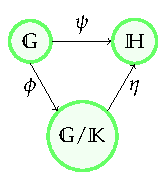
\includegraphics[scale=2]{../figures/FIT-fig.pdf} 	
      \caption{A diagrammatic interpretation of First Isomorphism Theorem.}
      \label{fig:FIT}   % Give a unique label
    \end{center}
\end{figure}
}

\frame{\frametitle{关于第一同构定理的直观认识.}
%Motivation of First Isomorphism Theorem. 20260511
\begin{figure}
	\begin{center}
		\input{../figures/g_to_h_mapping.tikz}
		\caption{关于第一同构定理的直观认识.}
		\label{fig:FIT_motivation}       % Give a unique label
	\end{center}
\end{figure}
%20260511
}

\frame{\frametitle{First Isomorphism Theorem.}
	\begin{block}{(证明思路.)}
		\begin{enumerate}
		\item Define $\eta: \mathbb{G}/\mathbb{K} \mapsto \psi(\mathbb{G})$ by $\eta(g \mathbb{K}) = \psi(g)$;
		
		\item Prove $\eta$ is well-defined;
		
		\item Prove that $\eta$ is a homomorphism and is a bijective map.
		\end{enumerate}
	\end{block}
}

\frame{\frametitle{First Isomorphism Theorem.}
	\begin{block}{(证明第一步.)}
		\begin{itemize}
		\item 定义映射$\eta: \mathbb{G}/\mathbb{K} \mapsto \psi(\mathbb{G})$为$\eta(g \mathbb{K}) = \psi(g)$。
		\end{itemize}
	\end{block}
}

\frame{\frametitle{First Isomorphism Theorem.}
	\begin{block}{(证明第二步.)}
		\begin{itemize}
		\item 证明$\eta$是良定义映射，即证明如果对于两个不同的$g_1, g_2 \in \mathbb{G}$，有$g_1 \mathbb{K}  =  g_2\mathbb{K} $，
				则$\eta(g_1 \mathbb{K} ) = \eta(g_2 \mathbb{K} )$。
				因为$g_1 \mathbb{K}  =  g_2\mathbb{K}$，则存在$k\in \mathbb{K}$使得$g_1 = g_2 k$，这仅仅利用了陪集相等的定义。因此：
				\[ \eta(g_1\mathbb{K} ) = \psi(g_1) = \psi(g_2 k) = \psi(g_2)\psi(k) = \psi(g_2) =  \eta(g_2\mathbb{K})\]
				请注意，上式中第四个等号之所以成立是因为$k\in \mathbb{K}$，而$\mathbb{K}$是$\psi$的Kernel，$k$必然映射到$\mathbb{H}$的单位元。
				这就证明了$\eta$映射独立于陪集代表元的选择。之所以$\eta$是唯一定义的，因为给定了$\psi$和$\phi$，而$\psi = \eta \phi$，且$\phi$是满射。
		\end{itemize}
	\end{block}
}

\frame{\frametitle{First Isomorphism Theorem.}
	\begin{alertblock}{(一个问题.)}
		确保$\eta$的唯一性，为什么需要$\phi$是满射?（课后练习！）
	\end{alertblock}
}

\frame{\frametitle{First Isomorphism Theorem.}
	\begin{block}{(证明第三步.)}
		\begin{itemize}
		\item 可证明$\eta$是同态且是双射。$\eta$是同态，因为：
				\begin{align*}
					\eta(g_1\mathbb{K} g_2 \mathbb{K}) &= \eta(g_1 g_2 \mathbb{K}) \\
					&=  \psi(g_1 g_2) \\
					&= \psi(g_1)\psi(g_2)\\
					&= \eta(g_1\mathbb{K})\eta(g_2\mathbb{K})
					\end{align*}
				$\eta$显然是满射，最后，只需证明$\eta$是单射。
		\end{itemize}
	\end{block}\pause
			
	\begin{alertblock}{(一点点提醒.)}
		为什么	$\eta$显然是满射?
	\end{alertblock}
}

\frame{\frametitle{First Isomorphism Theorem.}
	\begin{block}{(证明第三步.)}
		\begin{itemize}
		\item 证明$\eta$是单射。任取$g_1\mathbb{K}, g_2\mathbb{K}$，
				假设$\eta(g_1\mathbb{K} ) = \eta(g_2\mathbb{K} )$，
				则$\psi(g_1) = \psi(g_2)$。$g_1$和$g_2$是$\mathbb{G}$中两个不同的元素，所以
				\[\psi(g_1) = \psi(g_2 g_2^{-1} g_1) = \psi(g_2) \psi(g_2^{-1} g_1)\]
				即$\psi(g_2^{-1} g_1)$是$\psi(\mathbb{G})$的单位元，也即$g_2^{-1} g_1 \in \mathbb{K}$。
				所以$g_2^{-1} g_1\mathbb{K} = \mathbb{K} $，最后得到$g_1\mathbb{K} = g_2\mathbb{K}$。
		\end{itemize}
	\end{block}
}


%%%New examples added in 20201101
\frame{\frametitle{Example for First Isomorphism Theorem.}
\begin{exampleblock}{(Homomorphism from Cyclic Group.)} 
设$\mathbb{G}$是由生成元$g$生成的循环群。定义映射$\phi: \mathbb{Z} \mapsto \mathbb{G}$为$n \mapsto \ g^n$， $\forall n \in \mathbb{Z}$。
$\phi$是同态映射，因为：
\[\phi(m + n) = g^{m+n} = g^m g^n = \phi(m) \phi(n)\mbox{。}\]
$\phi$显然是满射。如果$\mathbb{G}$的阶为$m$，因为$g$是生成元，则$ord(g) = m$。
于是，$g^m = e$，且有$\operatorname{Ker}\; \phi = m \mathbb{Z}$。根据第一同构定理，则有：
\[\mathbb{Z} / \operatorname{Ker} \phi = \mathbb{Z} / m \mathbb{Z} \cong \mathbb{G}\mbox{。}\]
如果$\mathbb{G}$是无限阶，则$g$也是无限阶，则$\operatorname{Ker} \phi = \{ 0 \}$，则$\mathbb{Z}$与$\mathbb{G}$同构。
因此，两个循环群同构当且仅当它们有相同的阶。在同构的意义上，只有两种循环群：$\mathbb{Z}$和$\mathbb{Z}_n$。
\end{exampleblock}
}
%%%New examples added in 20191109
\frame{\frametitle{Example for First Isomorphism Theorem.}

\begin{exampleblock}{(Homomorphism from $\mathbb{Z}_p^*$ to $\mathbb{Z}_p^*$.)} 
	\label{exm:homo_zp}
	Let $p$ be a prime, $\mathbb{Z}_p^*$ is a cyclic group. Define a map $\phi: \mathbb{Z}_p^* \mapsto \mathbb{Z}_p^*$ by $\phi(g) = g^2$ for all $g \in \mathbb{Z}_p^*$. Then $\phi$ is a group homomorphism, since
	\[\phi(g_1  g_2) = (g_1 g_2)^ 2 = g_1^2 g_2^2 = \phi(g_1) \phi(g_2).\]
	Clearly $\phi$ is not onto, and $\operatorname{Ker} \phi = \{1, p-1\}$ is a normal subgroup of $\mathbb{Z}_p^*$. We know $\operatorname{Ker} \phi$ because we believe that the following equation
	\[x^2 \equiv 1 \pmod{p}\]
	has only two solutions, namely $1$ and $p-1$. 
	Check that $\mathbb{S} = \{ \phi(g): \mbox{for all}\; g \in \mathbb{Z}_p^*\} $ is a group. What is the order of $\mathbb{S}$? By the First Isomorphism Theorem, $\vert \mathbb{S} \vert = \vert \mathbb{Z}_p^* /  \operatorname{Ker} \phi \vert =  \vert \mathbb{Z}_p^* \vert /  \vert \operatorname{Ker} \phi \vert $.
	\end{exampleblock}
}

\frame{\frametitle{Example for First Isomorphism Theorem.}
	\begin{exampleblock}{(Homomorphism from $\mathbb{Z}_n^*$ to $\mathbb{Z}_n^*$.)} 
	%\label{exm:homo_zn}
	Let $n = p q$ be a composite integer, $p$ and $q$ are two primes, and $\mathbb{Z}_n^*$ is a group. Define a map $\phi: \mathbb{Z}_n^* \mapsto \mathbb{Z}_n^*$ by $\phi(g) = g^2$ for all $g \in \mathbb{Z}_n^*$. Then $\phi$ is a group homomorphism.  $\mathbb{S} = \{ \phi(g): \mbox{for all}\; g \in \mathbb{Z}_n^*\}$, if we know the order of $\operatorname{Ker}\; \phi$, then we know the order of $\mathbb{S} =\vert \mathbb{Z}_n^* \vert /  \vert \operatorname{Ker} \phi \vert $ by the First Isomorphism Theorem. How many solutions does the following equation have?
	\[ x^2 \equiv 1 \pmod{n}\]
	Unfortunately, we donot solve it until we learn CRT.
	\end{exampleblock}
	
}

\frame{\frametitle{一个值得记忆的结论.}
	\begin{block}{一个好用的结论.} 
	设$\phi: \mathbb{G}\mapsto \mathbb{H}$是一种群同态。$\phi$是单射当且仅当$\operatorname{Ker} \phi  = \{e\}$
	\end{block} \pause

	\begin{exampleblock}{证明.} 
	\begin{itemize}
		\item $\Rightarrow$: $\phi$是单射，显然$\operatorname{Ker}\; \phi  = \{e\}$。
		
		\item $\Leftarrow$: $\operatorname{Ker} \phi  = \{e\}$，根据第一同构定理，有$\mathbb{G} \cong \mathbb{G}/\operatorname{Ker} \phi \cong \phi(\mathbb{G})$。所以$\phi$是单射。	
	\end{itemize}
	
	\end{exampleblock}
	
}

\frame{\frametitle{例子-1.}
	\begin{block}{同构.} 
	设$\mathbb{G}$和$\mathbb{H}$是群。证明$\mathbb{G}\times \mathbb{H}$同构于$\mathbb{H}\times \mathbb{G}$ 
	\end{block} \pause

	\begin{exampleblock}{证明.} 
	\begin{itemize}
		\item 思路：构造第一同构定理的“三角关系”。并使得$\operatorname{Ker} \phi  = \{e\}$。	
	\end{itemize}
	
	\end{exampleblock}
	
}

\frame{\frametitle{例子-2.}
	\begin{block}{同构.} 
	设$\mathbb{H}$和$\mathbb{K}$是群$\mathbb{G}$的正规子群，且$\mathbb{H} \cap \mathbb{K} = \{e\}$。证明$\mathbb{G}$同构于$\mathbb{G}/\mathbb{H}\times \mathbb{G}/\mathbb{K}$的一个子群。 
	\end{block} \pause

	\begin{exampleblock}{证明.} 
	\begin{itemize}
		\item 思路：构造第一同构定理的“三角关系”。并使得$\operatorname{Ker} \phi  = \{e\}$。	
	\end{itemize}
	
	\end{exampleblock}
	
}
\iffalse
\frame{\frametitle{Example for First Isomorphism Theorem.}
\begin{exampleblock}{Homomorphism for Signed Group}
%\label{exm:signed_gr}
Let $n$ be a positive integer. For $x \in \mathbb{Z}_n$, we define $\vert x \vert$ as the absolute value of $x$, where $x$ is represented as a signed integer in the set $\{ -(n-1)/2, \cdots, (n-1)/2\}$.
From $\mathbb{Z}_n^*$, we define the set $\mathbb{G}^+$ as
\[\mathbb{G}^+  = \{ \vert x \vert : x \in \mathbb{Z}_n^*\} \]
with the following operations
\[ g \circ h = \vert g \cdot h \bmod{n} \vert,\]
where $g, h \in \mathbb{G}^+$. We know that $(\mathbb{G}^+, \circ)$ is indeed a group. What is the order of the group, and why?

\end{exampleblock}

}

\frame{\frametitle{Example for First Isomorphism Theorem.}
\begin{exampleblock}{Find the order of $\mathbb{G}^+$.}
\[\mathbb{G}^+  = \{ \vert x \vert : x \in \mathbb{Z}_n^*\} \]

\end{exampleblock}
\begin{exampleblock}{Answer.}

We observe that taking absolute value is a homomorphism, since
\[ \phi(x\cdot y) = \vert x \cdot y \vert = \vert x \vert \circ \vert y \vert = \phi(x) \circ \phi(y) \]

Since $-1 \in \mathbb{Z}_n^*$, $\operatorname{Ker} \phi = \{1, -1\}$. Then the oder of $\mathbb{G}^+$ is $\vert \mathbb{Z}_n^* \vert / 2 $.
\end{exampleblock}

}
\fi


\frame{\frametitle{Second Isomorphism Theorem.}
\begin{theorem}{(第二同构定理.)}
%\label{thm:sec_iso}
$\mathbb{H}$是群$\mathbb{G}$的子群（不必然是正规子群），$\mathbb{K}$是群$\mathbb{G}$的正规子群。
则$\mathbb{H} \mathbb{K}$是群$\mathbb{G}$的子群，$\mathbb{H}\cap \mathbb{K}$是$\mathbb{H}$的正规子群，
且
\[\mathbb{H} / (\mathbb{H}\cap \mathbb{K}) \cong \mathbb{H}\mathbb{K}/\mathbb{K}\mbox{。}\]
\end{theorem}
}

\frame{\frametitle{Correspondence Theorem.}
	\begin{block}{Correspondence Theorem. (对应定理)}
		Let $\mathbb{H}$ be a normal subgroup of a group $\mathbb{G}$. Then $\mathbb{H} \mapsto \mathbb{H}/\mathbb{H}$ is a one-to-one correspondence between the set of subgroups $\mathbb{H}$ containing $\mathbb{H}$ and the set of subgroups of $\mathbb{G}/\mathbb{H}$. Furthermore, the normal subgroups of $\mathbb{G}$ containing $\mathbb{H}$ correspond to normal subgroups of $\mathbb{G}/\mathbb{H}$.
	\end{block}
}

\frame{\frametitle{Correspondence Theorem.(对应定理)}
	\begin{exampleblock}{Understanding Correspondence Theorem.}
	\begin{enumerate}
    	\item What is the map $\mathbb{H} \mapsto \mathbb{H}/\mathbb{H}$?
		   \pause
		   
		 \item A map: $\{\mbox{the set of subgroups}\; \mathbb{H} \;\mbox{containing}\; \mathbb{H}\}  \mapsto \{\mbox{the set of subgroups of}\; \mathbb{G}/\mathbb{H}\}$ \pause
		  
		  \item To understand what is a subgroup of $\mathbb{G}/\mathbb{H}$?
	\end{enumerate}
	
	\end{exampleblock}
}

\frame{\frametitle{Correspondence Theorem.}
	\begin{block}{Proof ideas of the Correspondence Theorem.}
	\begin{enumerate}
	    \item $\mathbb{H}/\mathbb{H}$ is a subgroup of $\mathbb{G}/\mathbb{H}$;
	
    	\item The map $\mathbb{H} \mapsto \mathbb{H}/\mathbb{H}$ is one-to-one and onto;
		 
		 \item $\mathbb{H}$ is normal in $\mathbb{G}$, if and only if $\mathbb{H}/\mathbb{H}$ is normal in $\mathbb{G}/\mathbb{H}$.
	\end{enumerate}
	
	\end{block}
}

\frame{\frametitle{Third Isomorphism Theorem.}
\begin{theorem}{(第三同构定理)}
%\label{thm:third_iso}
$\mathbb{H}$和$\mathbb{K}$是群$\mathbb{G}$的正规子群，且$\mathbb{K}\subseteq \mathbb{H}$。则：
\[\mathbb{G}/ \mathbb{H} \cong \frac{\mathbb{G}/\mathbb{K}}{\mathbb{H}/\mathbb{K}}\mbox{。}\]
\end{theorem}
}

\frame{\frametitle{习题.}
\begin{block}{习题.}
\begin{itemize}

\item 证明：如果$\mathbb{H}$是群$\mathbb{G}$上指标为$2$的子群，则$\mathbb{H}$是$\mathbb{G}$的正规子群。
%（提示：出此题不是一次错误。）

\item 给定任意群$\mathbb{G}$，$\mathbb{H}$是群$\mathbb{G}$的正规子群。
请证明，如果群$\mathbb{G}$是阿贝尔群，则商群$\mathbb{G}/\mathbb{H}$也是阿贝尔群。

\item 给定任意群$\mathbb{G}$，$\mathbb{H}$是群$\mathbb{G}$的正规子群。
请证明，如果群$\mathbb{G}$是循环群，则商群$\mathbb{G}/\mathbb{H}$也是循环群。

 \item 设$p$和$q$是两个不同的素数，$\mathbb{G}$是阶为$pq$的阿贝尔群，请证明$\mathbb{G}$是循环群。
 
 \end{itemize}
 \end{block}
 }


\frame{\frametitle{习题讲解.}
	\begin{block}{习题.}
	设$p$和$q$是两个不同的素数，$\mathbb{G}$是阶为$pq$的阿贝尔群，请证明$\mathbb{G}$是循环群。
	\end{block}

	思路：找阶为$p$的群元$g_1 $和阶为$q$的群元$g_2$，则可知$ g_1 g_2$的阶是$pq$，则$\mathbb{G}$是循环群。\pause
\begin{proof}
不妨假设存在阶为$p$的群元$g_1$，$\mathbb{H}=\langle g_1 \rangle$为循环群。可得阶为$q$的商群$\mathbb{G}/\mathbb{H}$，它也必然为循环群。记
$\mathbb{G}/\mathbb{H}$的生成元是$ g_2 \mathbb{H}$。此时，$g_2$的阶不能是$1$。同时，$g_2$的阶不能是$p$，否则$ (g_2 \mathbb{H})^p = \mathbb{H}$。
如果$p < q$，则$g_2 \mathbb{H}$不能是生成元。如果$p > q$，则$q$整除$p$，这是不可能的！所以，$g_2$的阶只能是$q$或者$pq$，无论是什么情况，
$\mathbb{G}$都是循环群。
\end{proof}
 }

 \frame{\frametitle{关于第一同构定理运用的习题.}
\begin{block}{习题.}
\begin{itemize}

\item 证明：$\mathbb{GL}_n(R)/\mathbb{SL}_n(R)$与乘法群$\mathbb{R}^*$同构。

 \item 证明商群$\mathbb{R}/\mathbb{Z}$ 同构于圆圈群$\mathbb{O}$。
 
 \item 设$\phi: \mathbb{G}\mapsto \mathbb{H}$是一种群同态。请证明$\phi$是单射当且仅当$\operatorname{Ker} \phi  = \{e\}$。

 \item 给定有限阿贝尔群$\mathbb{G}$和正整数$n$，定义映射$\phi: \mathbb{G}\mapsto \mathbb{G}$为，$\forall g \in \mathbb{G}$，$\phi(g) = g^n$。
 请分析并证明，在什么条件下$\phi$会是一种单射？
 
 \end{itemize}
 \end{block}
 }

\end{document}
